\subsection{Reconstruction and Identification}
\label{sec:eleReco}
\par Electrons reconstructed in the ATLAS detecter are classified into {\it central} 
and {\it forward}, where central electrons are those within $|\eta|<2.5$ and 
forward electrons are those within $2.5<|\eta|<4.9$.
Since central electrons fall within the Inner Detector (ID) coverage, they make use 
of both the EM Calorimeter and the ID measurements while 
forward electrons rely just on the calorimeter information. As a result, calorimeter 
requirements on forward electrons are much more stringent than on central 
electrons.

\par Central electrons are reconstructed by matching energy clusters in the EM Cal 
to tracks in the ID, where a cluster is a group of calorimeter cells.
The slinding window algorithm (introduced in Section~\ref{sec:trigger}) is used 
to find these clusters by searching for calorimeter cells with energy deposits greater 
than 3~\GeV\ in windows of size $3\times 5$ calorimeter cells in $\eta\times\phi$\footnote{
The magnetic field bending plane in the ID is the $r\phi$ plane. The calorimeters may be subject 
to this field as well, albeit significantly weaker than in the ID}. The window 
is made larger in the $\phi$ direction to account for any magnetic field effects. This cluster 
search begins in Layer 2 of the EM Cal. Upon locating the cluster center in Layer 2 energy deposits 
in the corresponding pre-sampler, Layer 1 and Layer 3 are collected and summed. During Run I, using 
the sliding window algorithm, the efficiency for finding electrons with $\eT=7~\GeV$ was 95\% 
, 99\% for those with $\eT=15~\GeV$ and 99.9\% for those with $\eT=45~\GeV$~\cite{Aad:2014fxa}. 

\par Forward electrons are reconstructed using {\it topological clusters}~\cite{Lampl:2008zz}, whose clustering algorithm 
differs from the slinding window algorithm. Cells with large signal to noise ratio are used as seed and 
added to the cluster. The cluster grows by iteratively adding neighboring cells with a signal to noise ratio above a 
threshold slightly less than the seed threshold. Perimiter cells are added on the cluster by 
imposing an even lower energy threshold. This creates 3-dimensional clusters of varying energies. 
During Run I and Run II the seed threshold was 6~\GeV\ and both the neighbor and perimeter 
thresholds were 3~\GeV. This topological clustering scheme is known as EM 633, named after 
energy thresholds from seeds, neighbors and perimeters. 

\par Only tracks with $\pT>0.5~\GeV$, at least 
two hits in the Pixel Detector, at least seven total hits from the Pixel Detector and the SCT are 
considered for matching clusters in the EM Cal. These tracks are extrapolated from 
their last hit in either the Silicon Detectors or the TRT to Layer 2 of the EM Calorimeter.
A track and a cluster are considered a match if the cluster center and the track are within 
$|\Delta\eta|<0.05$ and $|\Delta\phi|<0.1$. The matching window in the $\phi$ coordinate 
is larger to allow for brehmsstrahlung losses due to the magnetic field. In the case of multiple tracks being matched 
to one cluster, preference is given to the tracks with most hits in the Silicon Detectors, based 
on the scoring method discussed in Section~\ref{sec:idtracks}, and the smallest  
$\Delta R$ between the track and the EM Calorimeter cluster. A central electron 
is considered reconstructed if a cluster is matched to a track, otherwise it is reconstructed as 
a photon. To minimize background, only electrons with at least 5~\GeV\ energy are reconstructed. 

\par Effectively, a reconstructed electron is characterized by the following : the cluster energy, the estimate 
of the energy deposited in the ID, EM Calorimeter pre-sampler energy, lateral cluster energy leakage and leakage 
of energy into the hadronic calorimeter. These five components are combined to estimate the total 
electron energy. At $0.5~\MeV$, the electron mass is taken as zero in the ATLAS detector. This approximation 
makes the total electron transverse energy equal to its \pT. 
For central electrons the ($\eta,\phi$) position is extracted from the tracks and  
for forward electrons it is extracted from the topological clusters.   

%\subsection{Identification} 
\par Reconstructed electrons are grouped into categories of several identification 
requirements. The variables that define these categories describe cluster (which in turn describes an electron shower) and 
track properties, as well as criteria used for track-cluster matching. 

\par Of prime importance in describing a shower is the extent of hadronic leakage and the lateral 
shower shape. Given that $\eThadone$ is the transverse energy in Layer 1 of the hadronic 
calorimeter behind the electron cluster, $\eThad$ is the transverse energy 
in the whole hadronic calorimeter section behind the electron cluster, $\eta_2$ is the 
$\eta$ position of the cluster in the EM calorimeter, and $\eT$ is the ratio of the 
cluster energy to $\cosh\eta_2$, the hadronic leakage is defined as 



\begin{equation}
\text{Hadronic Leakage} = \begin{cases} 
														\eThadone/\eT,& \mbox{if } |\eta_2|<0.8 \mbox{ and } |\eta_2|>1.37 \\ 
														\eThad/\eT, & \mbox{if } 0.8<|\eta_2|<1.37  
													\end{cases}
\end{equation}

The lateral shower shape is describe by, among many other variables, $R_\eta(37)$ 
defined as 

\begin{equation}
R_\eta(37) = E(237)/E(277)
\end{equation}
 
where $E(237)$ is the energy deposited in Layer 2 of the EM Calorimeter in a 
rectangle of size $3\times 7$ cell units in $\eta\times\phi$,
centered around the  cluster center. $E(277)$ is similarly the energy deposited 
in a rectangle of size $7\times7$ cell units. Hadronic leakage and lateral 
shower shapes are very efficient in rejecting $\pi^{\pm}$ decays and 
wide showers. To reject electrons from \pizero\ decays Layer 1 of the EM Calorimeter 
is used because of its finer granularity in $\eta$. As already discussed in Section~\ref{sec:trigger} 
\pizero\ decays result in two energy maxima. To search for these two energy maxima several 
variables are defined in a $0.125\times0.2$ $\Delta\eta\times\Delta\phi$ window around the cell 
with the highest energy deposit (the so-called hottest cell). Given that $E_{2nd}$ is 
the energy deposited in the second hottest cell, that $E_{min1}$ is the energy deposited 
in the cell with the least energy between the hottest and second hottest cell, 
$\Delta E = E_{2nd}-E_{min1}$ is an excellent variable for picking up the two 
energy maxima due to \pizero s.  

\par While calorimeter shower analysis significantly reduces backgrounds due to
charged hadron decays, background due to photon conversions are better reduced by 
track analysis. First, track quality requirements are demanded on candidate electron 
tracks: at least nine Pixel Detector hits where one of the hits must be in the B-layer, 
and the transverse impact parameter either with respect to the beamline or to the primary vertex 
is demanded to be less than a threshold value.  
To ensure track-cluster matching, in addition to the $\Delta\phi, \Delta\eta$ requirements 
discussed in the preceding section, the energy measurement from the calorimeter is 
compared to the \pT\ from the track bending. 

\par Categorization of electron identification is successive and inclusive. This means that first 
a category with minimal requirements is defined; latter categories are just sub-sets of the first 
category, with more stringent requirements. The categories are a trade-off between the signal 
efficiency (ratio of identified electrons to reconstructed electrons) and background 
rejection. Reconstructed electrons that pass the first category requirements are referred to 
as {\it loose}. Subsequent categories are referred to as {\it medium} and {\it tight}. 
In general loose electrons pass hadronic leakage and lateral shower shape requirements.   
Medium electrons are additionally pass shower shape requirements in Layer 1, reducing 
\pizero\ contamination. Tight electrons additionally use track quality and track matching criteria 
to reduce backgrounds due to photon conversions. 

\par Rather than directly imposing requirements 
on variables to distinguish between signal electrons and 
background objects, a multivariate technique is used for electron identification for analyses described in 
this text. The discriminant used is the log-likelihood function $\log{d_{\mathcal{L}}}$~\cite{ATLAS-CONF-2014-032}, 
where 

\begin{equation}
d_{\mathcal{L}} = \frac{\mathcal{L}_S}{\mathcal{L}_S + \mathcal{L}_B}, 
\label{eq:lglh}
\end{equation}

where $\mathcal{L}_{S,B}$ are likelihood functions on signal electrons and background objects 
respectively. The $\mathcal{L}_{S,B}$ are functions of probability density functions (pdf) obtained by training a 
multivariate classifier on signal electrons or background objects from Monte Carlo simulations  
using variables discussed in the preceding paragraphs as inputs. A generalization of 
a likelihood function is 

\begin{equation}
\mathcal{L}(\vec{x}) = \prod_{i=1}^{n} P_i(x_i)
\label{eq:lhf} 
\end{equation}

where $\vec{x}$ is a tuple of input variables and $P_i$ is a pdf for variable $i$. 
Categorization into identification categories is achieved by directly cutting on 
$\log{d_{\mathcal{L}}}$, where $d_{\mathcal{L}}$ is computed using successively 
more variables for loose, medium and tight categories.
 
\subsection{Measurement of efficiencies, corrections and uncertainties}
\label{sec:eleCorr}
\par This section quantifies the performance of the electron reconstruction and identification methods 
discussed so far. 

\subsubsection{Efficiency}
\par Electron identification and reconstruction suffers from inefficiencies due 
to detector limitations. These inefficiencies are measured in data and in Monte Carlo 
simulation and compared, ultimately correcting the Monte Carlo simulation predictions. 

\par The total efficiency of reconstructing and identifying electrons for use in an 
analysis can be factorized into its major components as  

\begin{equation}
\epsilon_{total} = \epsilon_{reco} \times \epsilon_{id} \times \epsilon_{trigger} \times \epsilon_{isolation}
\end{equation}

where $\epsilon_{reco}$ is the efficiency of reconstructing an electron once an 
electromagnetic cluster is found in the EM Calorimeter, and $\epsilon_{id}$ is the 
efficiency of categorizing the reconstructed electron as loose, medium or tight.
$\epsilon_{trigger}$ is the efficiency of an identified electron to pass a particular 
trigger and $\epsilon_{isolation}$ is the efficiency of an electron that has passed the trigger 
to pass an isolation selection criteria. These efficiencies are computed successively. For example, 
an electron that passes the trigger selection must have also passed identification, and 
reconstruction. $\epsilon_{reco}$ is particularly 
important because it quantifies track reconstruction and track-cluster matching. 
Electrons, at a mass of $0.5~\MeV$, suffer more from brehmsstrahlung as they 
traverse material in the ID than heavier particles. This results in unpredictable 
deviations in the electron track path in the ID, leading to relatively 
poor reconstruction. $\epsilon_{id}$ on the other hand quantifies the perfomance 
of the Log Likelihood function described in the previous section. This section 
discusses the method for extracting $\epsilon_{id}$ and $\epsilon_{reco}$. 

\par For studies discussed in this text $\epsilon_{id}$ and $\epsilon_{reco}$ were extracted from \Zee\ and 
and \Jee\ events in data to cover a wide electron $\pT$ range. 
In both these cases, the {\it tag-and-probe} method was utilized~\cite{Aad:2011mk}. Here, one 
electron was fully reconstructed and identified with the highest efficiency 
possible. This is known as the tag electron. The other electron was used to 
probe the selection efficiency in question by requiring it to satisfy conditions 
either before or after the selection was been applied. For \Zee\ events, 
the tag electron was tightly identified, matched to a tight trigger electron, had $\eT>20~\GeV$ and  
lied outside the calorimeter transition region ($1.37<|\eta|<1.52$).
For \Jee\ events the tag electron was tightly identified, matched to a tight 
trigger electron object and have $\eT>5~\GeV$. In both cases, a tag object was required 
to be present, with a quality dependent on the type of efficiency being measured. 
For \Zee\ events, \mT\ of the probe object and the tag electron was required to lie between 80 and 100~\GeV.

\par To evaluate systematic uncertainties in the efficiencies being measured, several 
efficiency measurements with variations on the event selection criteria were 
performed. For example, the tag electron was modified or the background estimation 
was varied.  

\par For $\epsilon_{id}$ a reconstructed electron was used as a probe.
In \Zee\ events this probe electron had to have $\eT>10~\GeV$. 
Measurements were extracted from two dimensions: electron \eT\ and  
$\eta$. The decision to bin measurements in $\eta$ was motivated by the fact that brehmsstrahlung 
losses depend on the amount of material that the electron traverses in the ID, which is in turn 
dependent on $\eta$. Results from \Zee\ and \Jee\ events were combined, including systematic 
uncertainties. Figure~\ref{fig:idEff} shows these efficiencies binned 
in \eT\ and $\eta$, in both Monte Carlo simulation and data.  
In general, Monte Carlo simulation modelling agrees reasonably with data. 
The background rejection was also observed to be as large as 400. 

\begin{figure}[h]
\begin{subfigure}{0.5\textwidth}
   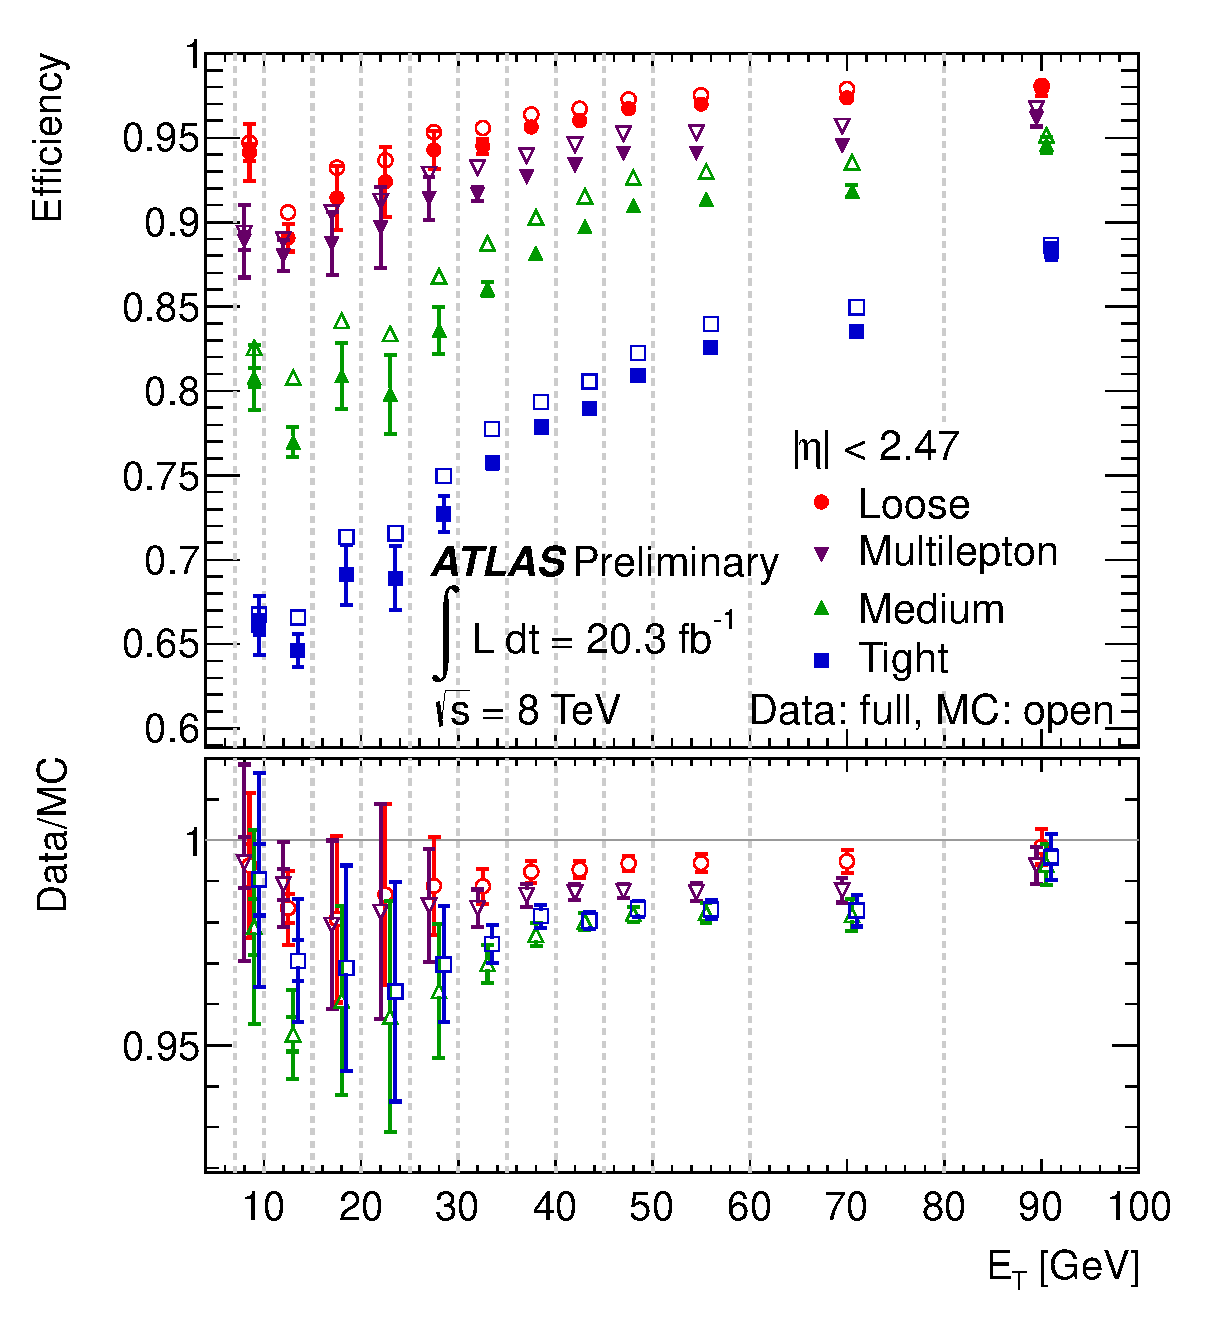
\includegraphics[width=\textwidth]{figures/can_CompEffDataMCLooseMultileptonMediumTightall_0.eps}
	\caption{\eT}
\end{subfigure} % 
\begin{subfigure}{0.5\textwidth}
   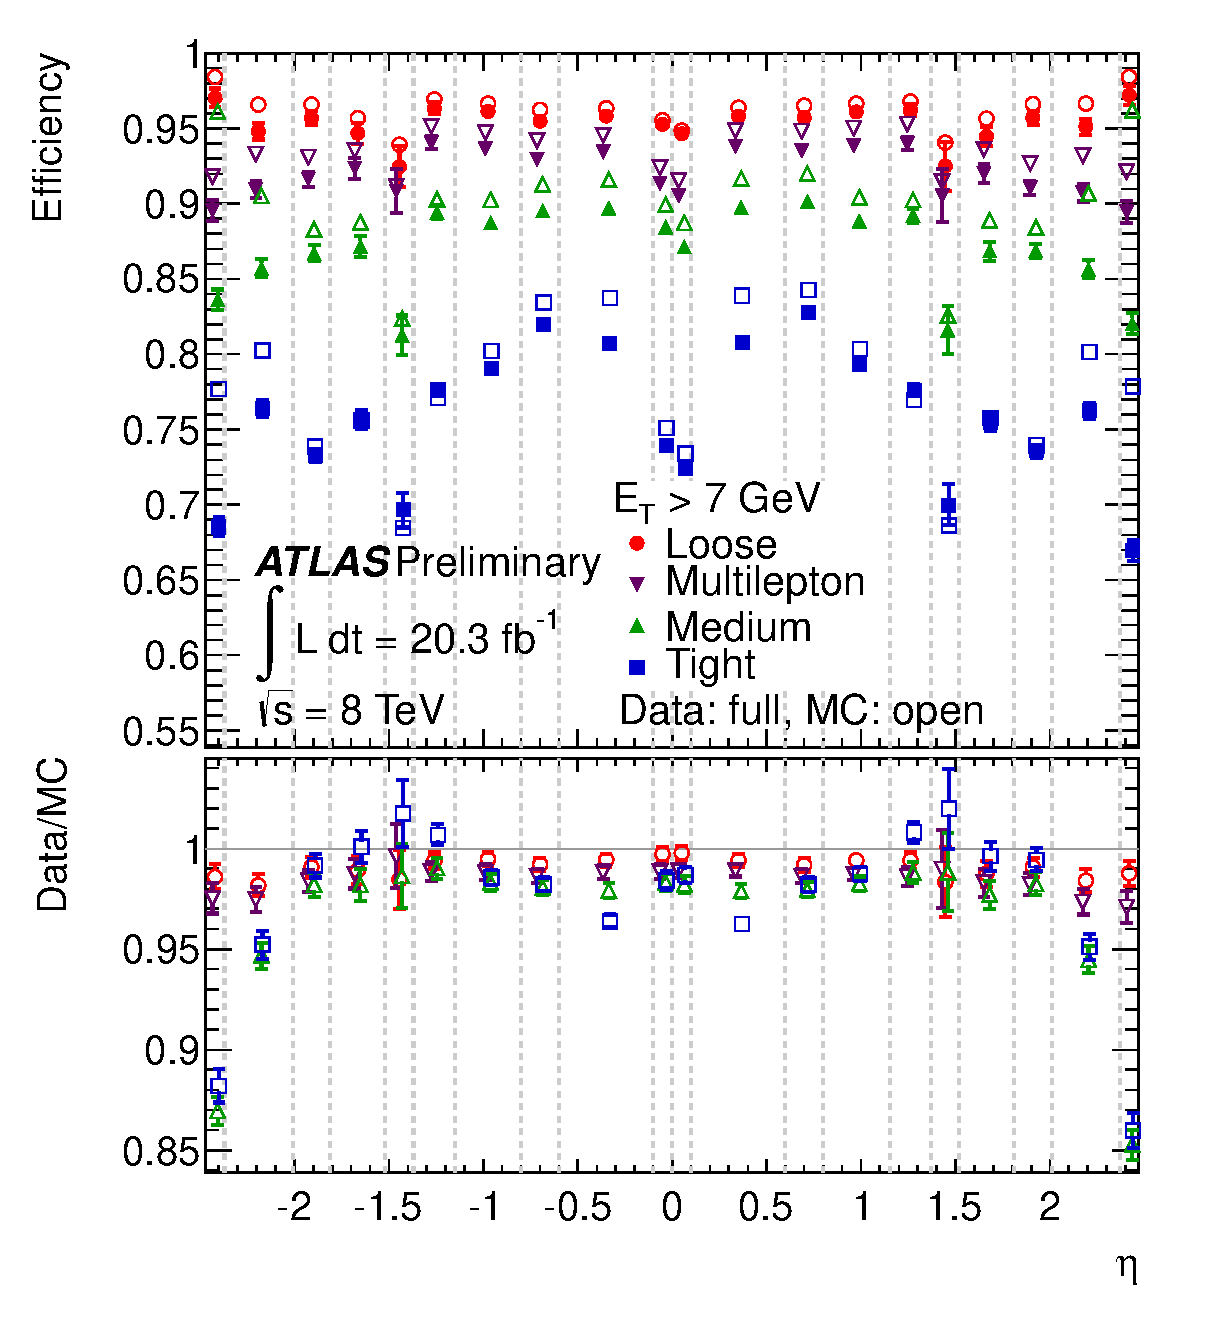
\includegraphics[width=\textwidth]{figures/can_CompEffEtaDataMCLooseMultileptonMediumTightone_0.eps}
	\caption{$\eta$}
\end{subfigure}
\caption{Plots of electron identification efficiencies during Run 1, binned in \eT, and $\eta$. 
Taken from Ref~\cite{Aad:2011mk}}
\label{fig:idEff}
\end{figure}

\par To measure $\epsilon_{reco}$ with \Zee\ events an EM cluster was taken as the probe 
object. This cluster was required to be isolated from electrons, to reduce backgrounds from 
photons. Measurements were binned in \eT\ and $\eta$. Figure~\ref{fig:recoEff} shows the 
measurements obtained data and Monte Carlo simulations. Overall there is reasonable 
agreement between data and Monte Carlo predictions. For the data set used for the analysis in this 
text (2012), the reconstruction efficiencies are at least 90\%.   

\begin{figure}[h]
\begin{subfigure}{0.5\textwidth}
   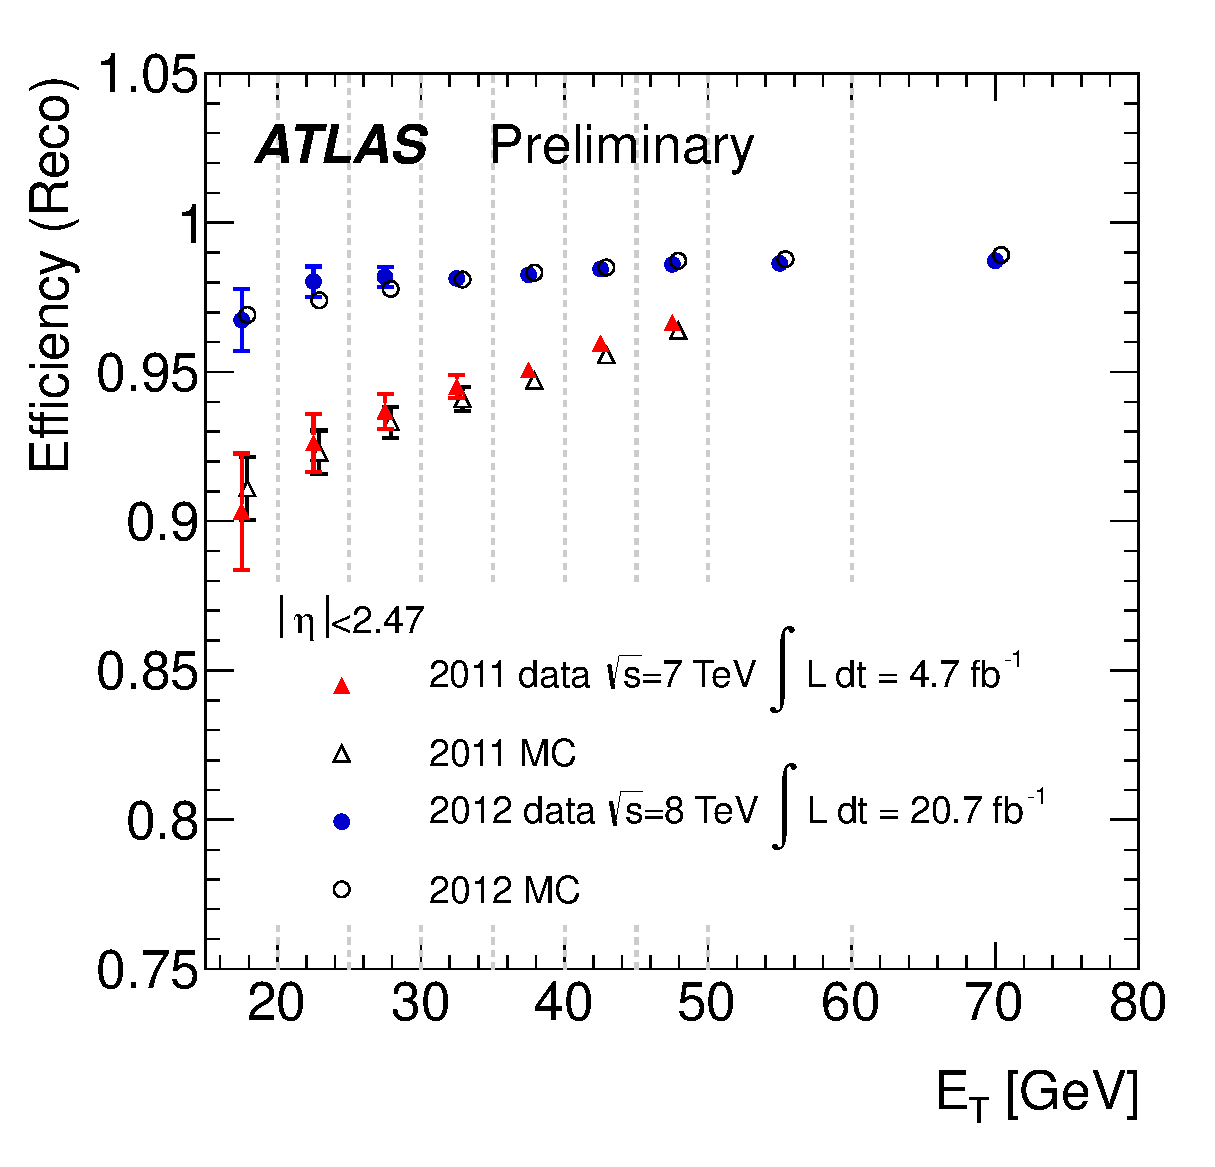
\includegraphics[width=\textwidth]{figures/Reco_et.eps}
	\caption{\eT}
\end{subfigure} % 
\begin{subfigure}{0.5\textwidth}
   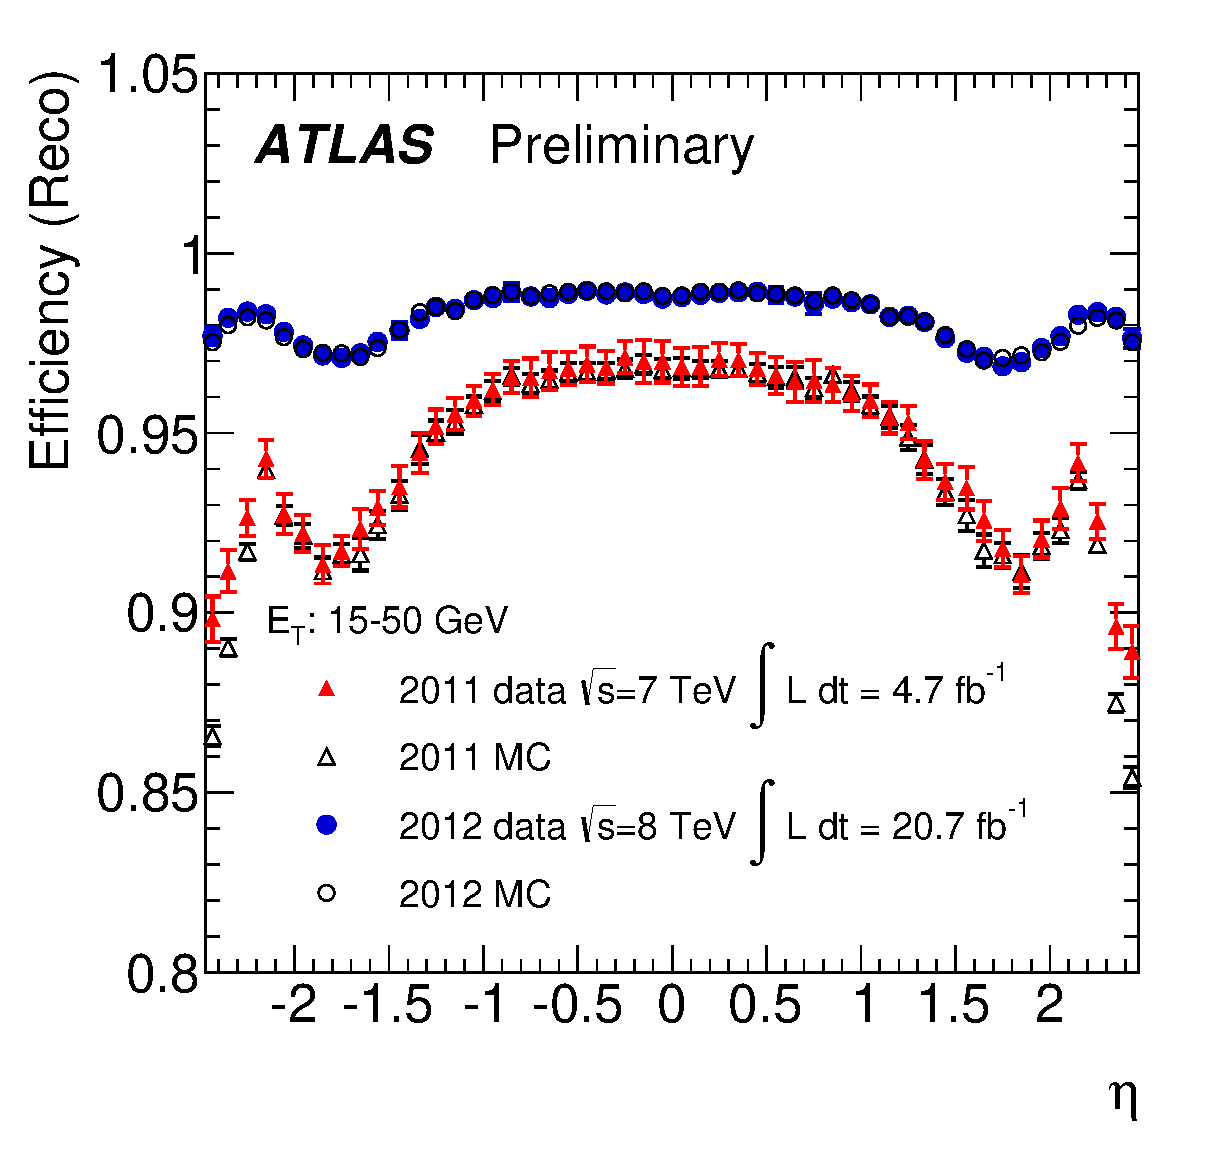
\includegraphics[width=\textwidth]{figures/Reco_eta.eps}
	\caption{$\eta$}
\end{subfigure}
\caption{Plots of electron reconstruction efficiencies during Run 1, binned in \eT, and $\eta$. 
 Taken from Ref~\cite{Aad:2011mk}}
\label{fig:recoEff}
\end{figure}


\subsubsection{Calibration}
\par Electron energy loss in the material upstream or beyond the Lar calorimeters, or outside 
the EM cluster in $\eta$ and $\phi$, was corrected for using dedicated calibration schemes. 

\par To determine these calibration parameters, a Boosted Decision Tree (BDT) was trained on Monte Carlo 
simulation to predict the true electron energy $E_{\text{true}}$ from variables such as the EM cluster 
energy, position, leakages, and ratios of cluster energies in different layers of the Lar calorimeters. 
The training was categorized by $\eT$ and $\eta$, whose binning were chosen to optimize energy responses 
in different regions of phase space. Calibration using this BDT was shown to improve energy 
resolutions by 10\%~\cite{Aad:2014nim}.  

\par Several other corrections were applied to electron candidates after the BDT calibration. For example, 
the energy scales in the first and second layers of the Lar calorimeters were equalized between data 
and Monte Carlo simulation. After that, the overall electron energy response in data was 
calibrated so that it agreed with the expectation from simulation using $\Zee$ events. These calibrations 
were categorized in $\eta$. The sensitivity of the results was evaluated by varying the event selection 
in data, and the quality of the electrons used. 

\par After all these calibrations were applied the agreement between 
data and Monte Carlo simulation was validated in $\Jee$ events, to test the performance in 
a different $\eT$ regime. Figure~\ref{fig:calibVal} shows the invariant masses of the $ee$ 
system in $\Jee$ and $\Zee$ events, covering different $\eT$ regimes. In the \Zee\ case, distributions from data was 
compared to those from calibrated Monte Carlo simulation and uncalibrated Monte Carlo simulation.  
In the \Jee\ case, some of the background component was data-driven, so the calibrated data was 
compared to the sum of Monte Carlo simulation and the data-driven background. 
In both cases, agreement was within 2\%. 

\begin{figure}[h]
\begin{subfigure}{0.5\textwidth}
   \includegraphics[width=\textwidth]{figures/JPsiPlot.pdf}
	\caption{\Jee}
\end{subfigure} % 
\begin{subfigure}{0.5\textwidth}
   \includegraphics[width=\textwidth]{figures/LineShapePlot_NotZoomed_ForPaper_v3.pdf}
	\caption{\Zee}
\end{subfigure}
\caption{Plots of the invariant mass of the $ee$ system in $\Jee$ and $\Zee$ events in data, calibrated and uncalibrated 
 Monte Carlo simulation. Taken from Ref~\cite{Aad:2014nim}}
\label{fig:calibVal}
\end{figure}

\par Uncertainties in the electron energy scale stemmed from several sources. For example, uncertainties associated 
with calibrating individual Lar layers reached 0.15\%. Those associated with the distribution of material upstream
 the Lar reached 0.3\%. Added in quadrature, overall the uncertainty on energy scale varied from 0.04\% to 0.4\% depending 
on $\eta$. Forward electrons suffered the most. The relative uncertainty on energy resolution was better than 10\% for 
50~\GeV\ electrons, and asymptotically rose to 40\% for higher energies.   
